\documentclass{gescons}

\genre {Entrevista}
\author{Alexandre Zaslavksy}
\title{Autoexperimentação Conscienciológica: Método dos Autotestes Experienciais, Pró-evolutivos e~Multidimensionais}
\paginaurl{https://www.youtube.com/live/csg8Ei53wxQ}

\begin{document}
    \makeentrevistatitle

    \coverart{back/alexandre}
    
    \begin{multicols}{2}

\begin{center}
    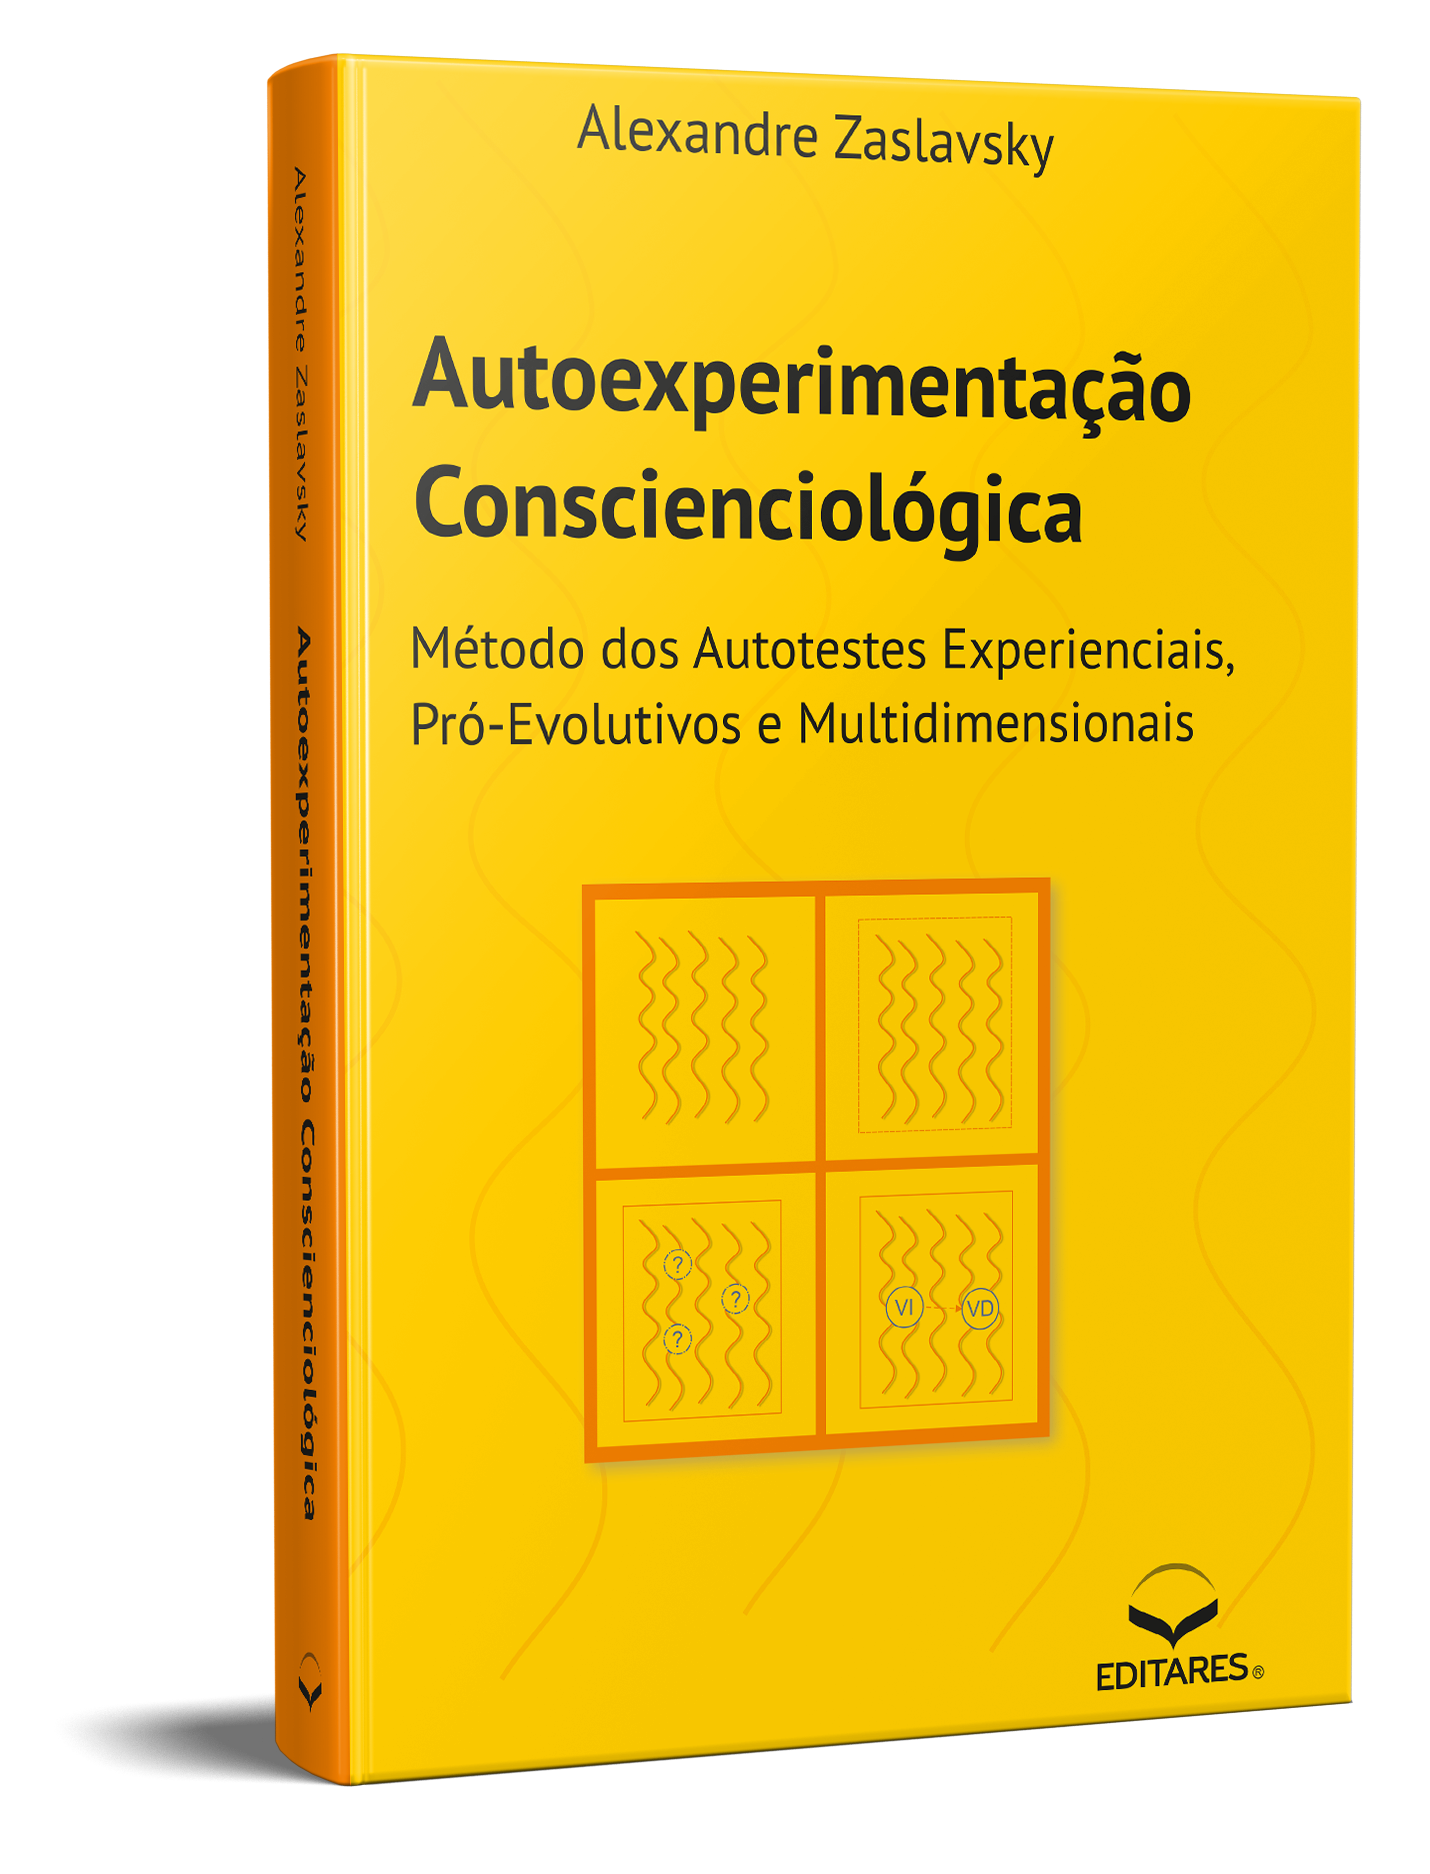
\includegraphics[width=4cm]{articles/entrevista/mockups/Alexandre-Zas}
\end{center}

\textbf{1. Qual foi a~motivação para a~escrita da obra? Por que a~definição deste tema para publicação de um livro?}

Desde que cheguei na Conscienciologia, o~seu novo paradigma científico, abrangendo a~multidimensionalidade dentre outros fatores, foi um grande motivador para mim. Assumi o~tema das bases da nova cientificidade conscienciológica, inicialmente de modo mais filosófico ou teórico e,~após, de modo mais conceitual e~teático. O~livro é~o~resultado dessas pesquisas sobre as bases teáticas da ciência Conscienciologia. A~autoexperimentação conscienciológica considero ser o~método científico mais básico e,~portanto, mais prioritário a~ser descrito, desenvolvido e~divulgado, tendo em vista o~público que se identifica com essa tarefa proexológica.

\textbf{2.       Quais foram as principais percepções, intra e~extrafísicas, durante a~pesquisa e~a~escrita da obra? E~posterior ao lançamento?}

A pesquisa e~escrita da obra foram muito ricas em autoexperimentos conscienciológicos, os quais são suscitados pelas experiências cotidianas e~são insitamente multidimensionais. A~interação com a~prática da tenepes também foi muito proveitosa, trazendo múltiplas inspirações de ideias, abordagens e~formulações mais assertivas interassistencialmente, seja diretamente com ideias ou indiretamente mediante parapercepções de processos extrafísicos. Foi possível observar na fase final da escrita o~aporte mais ostensivo de amparadores extrafísicos, auxiliando a~obter a~finalização propriamente da gescon, com a~qualidade necessária. Além disso, as trocas contínuas com colegas pesquisadores, mencionados nos Agradecimentos, foi de enorme auxílio ao longo da elaboração do trabalho.



\textbf{3.       Qual o~maior aprendizado com a~escrita desta obra?}

As revisões heterocríticas são imprescindíveis para a~qualificação do texto. Sem dúvida, considerar cuidadosamente as revisões recebidas, permitiu aprofundar e~amadurecer o~conteúdo do livro de modo incomparável com a~versão inicial. Além disso, a~publicação de uma obra tarística supõe a~assunção de autorresponsabilidade. Não é~possível depender da validação de autoridades para se trazer novas ideias a~público. O~autor chega a~determinado acúmulo de experiências e~conhecimentos que cabe tão somente a~ele, dentro dos parâmetros exigidos pela editora, assumir a~autoria publicamente. Portanto, o~primeiro maior aprendizado foi com a~interdependência e~o~segundo com a~independência relativa.


\textbf{4.       O~que poderia dizer como incentivo para que mais pesquisadores invistam na publicação de obras conscienciológicas?}

A escrita de uma obra conscienciológica é~uma oportunidade evolutiva inigualável. Desde a~escolha da temática, passando pelas experiências no decorrer da pesquisa e~escrita, até a~configuração final da obra, tudo isso expressa o~perfil específico do autor, conforme o~seu momento evolutivo. E~também, é~claro, atende ao grupo de afins que compartilha esse perfil. Além disso, apenas o~livro permite abordar as temáticas prioritárias no seu conjunto, de modo mais completo, seja na quantidade e~também na profundidade necessária. Publicar um livro enquanto gescon, portanto, é~possivelmente a~técnica evolutiva mais precisa e~eficaz.

\begin{pullquote}
``A escrita de uma obra conscienciológica é~uma oportunidade evolutiva inigualável.''
\end{pullquote}

        
    \end{multicols}
\end{document}
